\subsection{Obrácený oscilátor v jámě}
	Uvažujte jednorozměrný potenciál daný předpisem
	\begin{equation}\label{eq:InverseHarmonicOscillator}
		V(q)=
			\begin{cases}
				-\frac{1}{2}kq^{2} & -a\leq q\leq a\\
				\infty & \abs{q}>a
			\end{cases}
	\end{equation}
	(obrácený harmonický oscilátor v nekonečně hluboké pravoúhlé jámě, viz obrázek~\ref{fig:InverseHarmonicOscillator}(a)).
	Spočítejte hustotu kvantových hladin.
	
	\begin{solution}
		Při výpočtu se bude využívat vztah~\eqref{eq:LevelDensity1D}.
		
		\begin{enumerate}
			\item $E<0$:		
				V tomto případě je
				(díkz sudosti potenciálu stačí počítat jen v oblasti $x>0$ a výsledek zdvojnásobit):
				\begin{align*}
				\Omega(E)
					&=2\sqrt{2m}\int_{\sqrt{\frac{2\abs{E}}{k}}}^{a}\frac{1}{\sqrt{-\abs{E}+\frac{1}{2}kq^{2}}}\d q\\
					&=2\sqrt{\frac{2m}{\abs{E}}}\int_{\sqrt{\frac{2\abs{E}}{k}}}^{a}\frac{1}{\sqrt{\frac{k}{2\abs{E}}q^{2}-1}}\d q
					&&\equationcomment{b=\sqrt{\frac{k}{2\abs{E}}}\,q & \d q=\sqrt{\frac{2\abs{E}}{k}}\d b}\\
					&=\frac{4}{\omega}\int_{1}^{\sqrt{\frac{k}{2\abs{E}}}\,a}\frac{1}{\sqrt{b^{2}-1}}\d b
					&&\equationcomment{b=\cosh{z} & \d b=\sinh{z}\d z}\\
					&=\frac{4}{\omega}\int_{0}^{\arccosh\left(\sqrt{\frac{k}{2\abs{E}}}\,a\right)}
						\frac{\sinh{z}}{\sqrt{\cosh^{2}{z}-1}}\d z\\
					&=\frac{4}{\omega}\,\arccosh\left(\sqrt{\frac{k}{2\abs{E}}}\,a\right),
				\end{align*}
				kde $-\frac{1}{2}ka^{2}\leq E\leq0$.
				
				Hustota hladin je tedy
				\begin{equation*}
					\rho(E)
						=\frac{2}{\pi\hbar\omega}\,\arccosh\left(\sqrt{\frac{k}{2\abs{E}}}\,a\right).
				\end{equation*}
			
			\item $E>0$
			
			Podobným postupem jako v případě záporné energie dostaneme
			\begin{equation*}
				\rho(E)
					=\frac{2}{\pi\hbar\omega}\,\arcsinh\left(\sqrt{\frac{k}{2\abs{E}}}\,a\right).
			\end{equation*}				
		\end{enumerate}
		
		\begin{figure}[!htbp]
			\begin{subfigure}{0.45\linewidth}
				\centering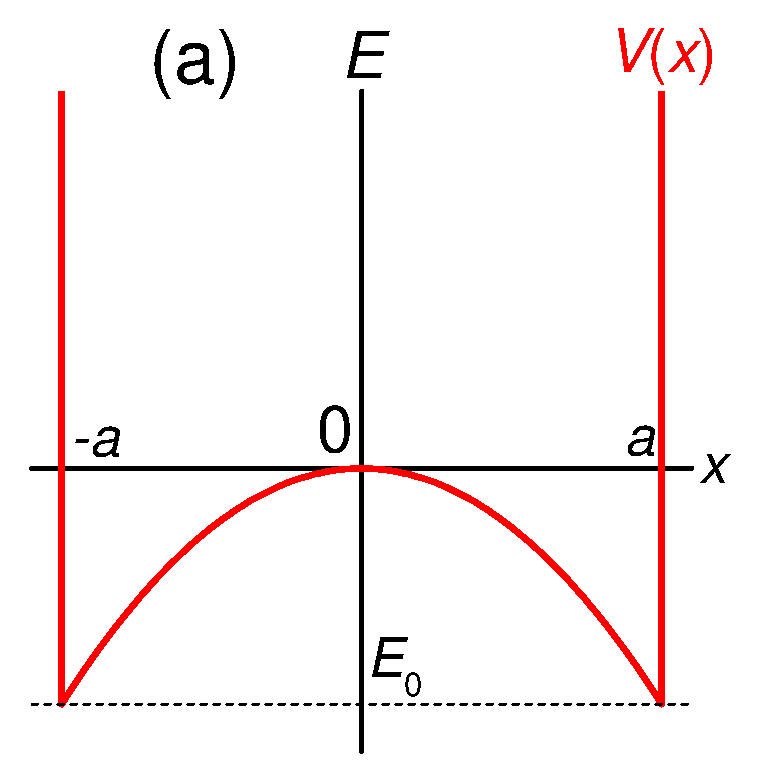
\epsfig{file=iho.eps,width=\linewidth}
			\end{subfigure}
			\hfill
			\begin{subfigure}{0.45\linewidth}
				\centering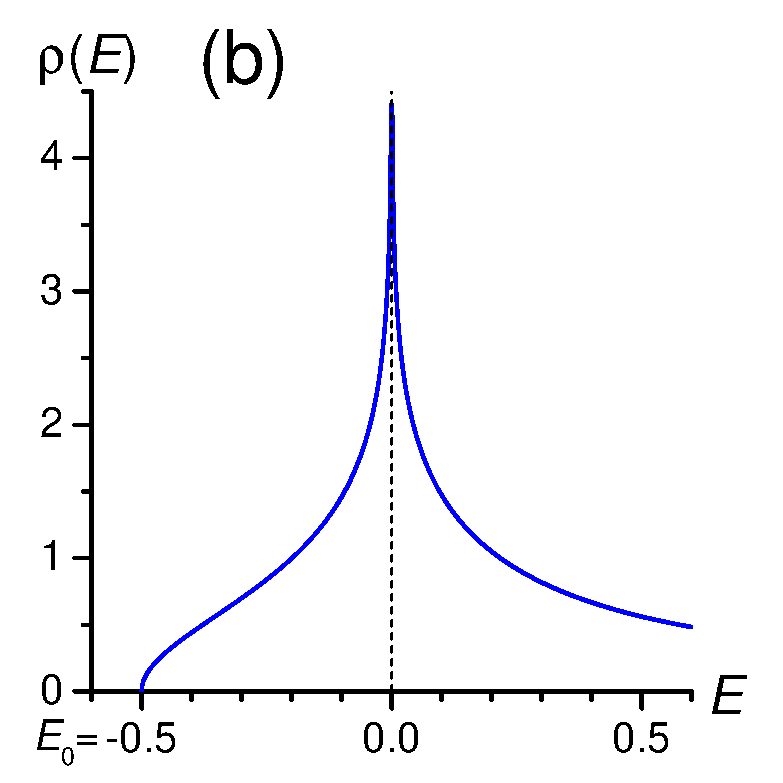
\epsfig{file=ihodensity.eps,width=\linewidth}
			\end{subfigure}
			\scaption{
				(a) Schéma potenciálu~\eqref{eq:InverseHarmonicOscillator}.
				(b) Hustota kvantových hladin při volbě $a=\hbar=m=k=1$.
			}
			\label{fig:InverseHarmonicOscillator}
		\end{figure}
		
		Výsledná hustota hladin je znázorněna na obrázku \ref{fig:InverseHarmonicOscillator}(b).
		Je vidět, že pro $E=0$ hustota diverguje.
		To je důsledek skutečnosti, že v klasickém případě je bod obratu při této energii v bodě $q=0$
		patologický, $V''(q=0)=0$, a patologická je i jediná možná trajektorie při této energii (její perioda je nekonečná).
    \end{solution}
